\documentclass[xcolor=dvipsnames,aspectratio=169,t]{beamer}
  % t means frames are vertically centered to the top
\usepackage{slides-header}

\title{Dot Product, Length, and Orthogonality}

\begin{document}
\maketitle

\begin{frame}{Calculating the Length of a Vector}
  \begin{columns}[T]
  \column{0.5\tw}
  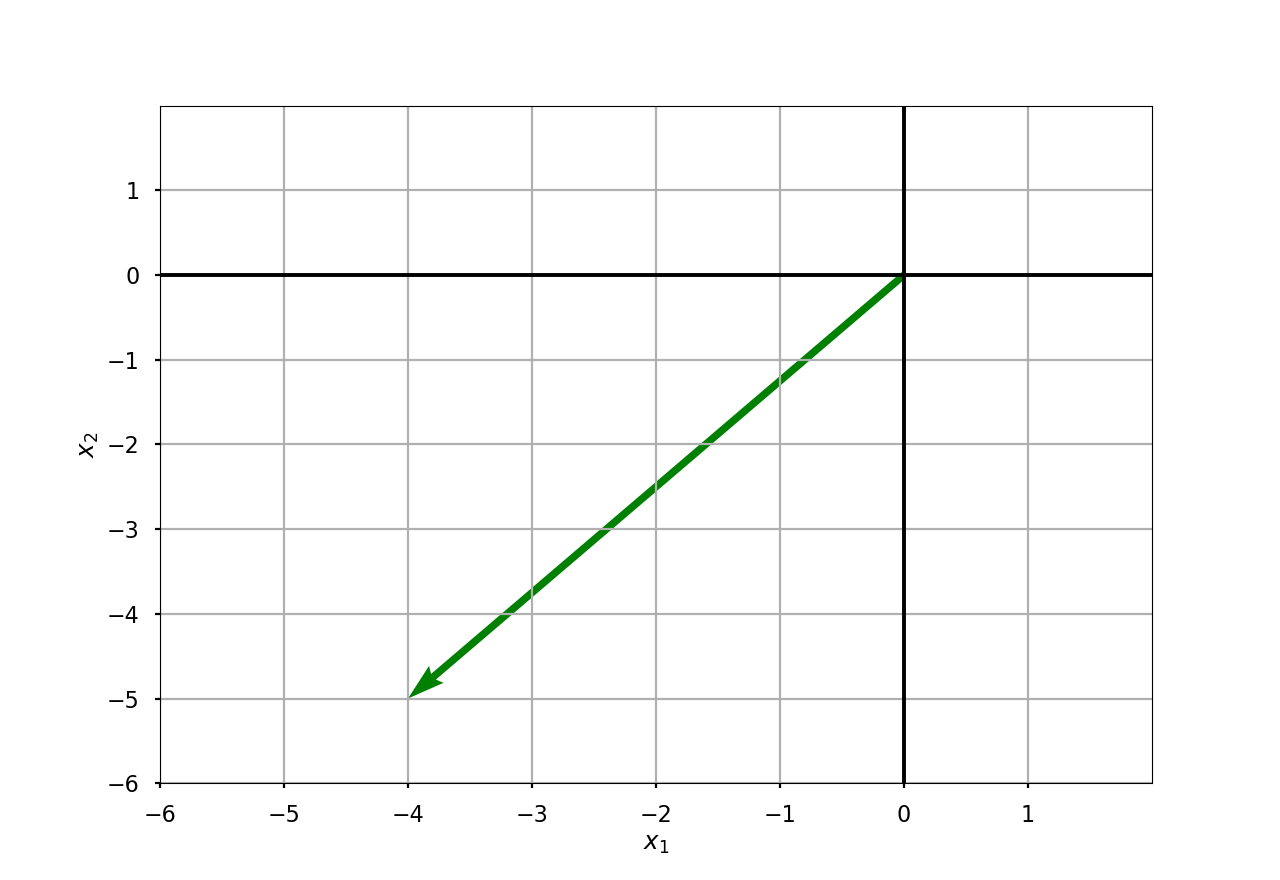
\includegraphics[width=0.6\tw]{images/fig-dist1.png}
  
  \qquad {\small $\v=(-4,-5)$
  \medskip
  
  Use the Pythagorean theorem:
  \smallskip
  
  \quad $\| \v \| = \sqrt{v_1^2+v_2^2} =  \sqrt{(-4)^2+(-5)^2} = \sqrt{41}$
  }

  \column{0.5\tw}
  \pause
  
  \vspace*{4em}
  
  Let $\w=(1,2,3)$ be a vector in $\R^3$.
  
  {\small \[ \| \w \| = \sqrt{w_1^2+w_2^2+w_3^2} =   \sqrt{1^2+2^2+3^2} = \sqrt{14} \]}
  \end{columns}
  \medskip
  
  \pause
  \bbox
  The \alert{length} (or \alert{norm}) of $\v$ is the nonnegative scalar \alert{$\dsty \| \v \| = \sqrt{v_1^2 + v_2^2 + \ldots + v_n^2}$}.
  \ebox
\end{frame}


\begin{frame}{The Dot Product}
  \begin{definition}
    Let $\u$ and $\v$ denote two $n \times 1$ column vectors in $\R^n$. 
    The \alert{dot product} %(or the \alert{inner product})
    of $\u$ and $\v$ is the scalar% 
    \[ \u \cdot \v = u_1v_1 + u_2 v_2 + \ldots + u_nv_n = \sum_{i=1}^n u_iv_i 
    \pause
    = \u^T \v 
    = \begin{bmatrix} u_1 & u_2 & \ldots & u_n \end{bmatrix} 
      \begin{bmatrix} v_1 \\ v_2 \\ \vdots \\ v_n \end{bmatrix}.
    \]
  \end{definition}
  \bigskip

  \pause
  \blue{Example.}
  \smallskip
  
  If $\u = \begin{bmatrix} 2 \\ -5 \\ 1 \end{bmatrix}$ and 
     $\v = \begin{bmatrix} 6 \\ 2 \\ -7 \end{bmatrix}$ in $\R^3$, 
     then $\u \cdot \v = (2)(6)+ (-5)(2) + (1)(-7) = -5$.
\end{frame}


\begin{frame}{Properties of the Dot Product}

  \begin{theorem}
  Let $\u$, $\v$, and $\w$ be vectors in $\mathbb{R}^n$, and let $c$ be a scalar. Then \smallskip
  \bb[(a)]
  \ii $ \u \cdot \v  =  \v \cdot \u $. \medskip
  \ii $(\u + \v) \cdot \w = (\u \cdot \w) + (\v \cdot \w)$. \medskip
  \ii $(c \u) \cdot \v = c(\u \cdot \v) = \u \cdot (c \v)$. \medskip
  \ii $\v \cdot \v \geq 0$, and $\v \cdot \v =0$ if and only if $\v = \mathbf{0}$. \medskip
  \ee
  \end{theorem}

  \bigskip

  \pause
  \begin{definition}
  The \alert{length} (or \alert{norm}) $\| \v \|$ of $\v$ is the nonnegative scalar $\| \v \| = \sqrt{ \v \cdot \v}$.
  \end{definition}
\end{frame}


\begin{frame}{Scaling Vectors}

\begin{columns}[T]

\column{0.3\tw}

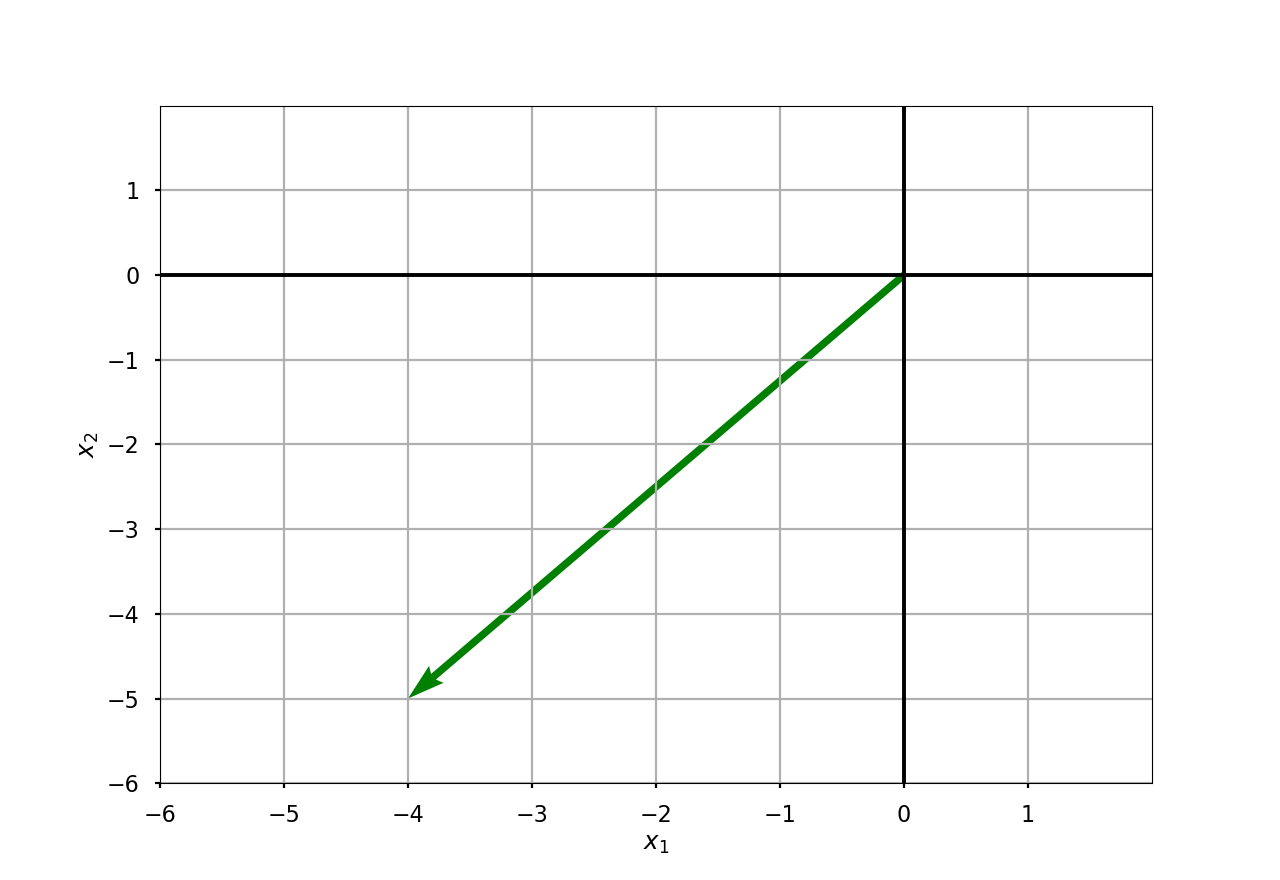
\includegraphics[width=0.95\tw]{images/fig-dist1.png}

\column{0.7\tw}

\bb
\ii Find a vector $\w$ that has the same direction as $\v=(-4,-5)$ but is twice as long.
\ii Find a vector $\u$ that has the same direction as $\v$ that has length 1.
\ee

\pause
\bbox
Let $c$ be a scalar. Then $\| c \v \|= |c|\ \| \v \|$. 
\ebox
\end{columns}

\pause
\bb
\ii Let $\w = 2(\v) = \begin{bmatrix} -8 \\ -10 \end{bmatrix}$ has the same direction as $\v$ and is twice as long.
\ii Note that $\|\v\| = \sqrt{41}$. If we scale $\v$ by a factor of $1/\| \v \|$, then we will obtain a vector in the same direction as $\v$ with magnitude equal to 1:
\[ \u = \frac{1}{\|\v\|} \v = \frac{1}{\sqrt{41}} \v = \begin{bmatrix} -4/\sqrt{41} \\ -5/\sqrt{41} \end{bmatrix}; \qquad \|\u\| = 1 \]
\ee

\end{frame}


\begin{frame}{Normalizing Vectors}
  \begin{definition}
    A vector $\u$ whose length is $1$ is called a \alert{unit vector}.
    The process of creating a unit vector $\u$ in the same direction as a vector $\v$ is called \alert{normalizing} $\v$.
    We have \[ \u = \frac{1}{\| \v \|} \v .\]
  \end{definition}
  \bigskip

  \pause
  \blue{Example.}\medskip

  Compute the unit vector in the direction of $\v = \begin{bmatrix} 1\\ 2\\ 3\end{bmatrix}$.
  \pause
  $ \u = \displaystyle\frac{1}{\| \v \|} \v 
  = \displaystyle\frac{1}{\sqrt{14}}\begin{bmatrix} 1\\ 2\\ 3\end{bmatrix}
  =\begin{bmatrix} 1/\sqrt{14} \\ 2/\sqrt{14} \\ 3/\sqrt{14} \end{bmatrix}$.
\end{frame}


\begin{frame}{Distance between two vectors}
  \begin{columns}[T]
  \column{0.6\tw}
  \begin{example}
  Compute the distance between \colorg{$\u = \begin{bmatrix} 6 \\ 6 \end{bmatrix}$} and \alert{$\v = \begin{bmatrix} 4 \\ 2 \end{bmatrix}$}.
  \end{example}

  \column{0.4\tw}
  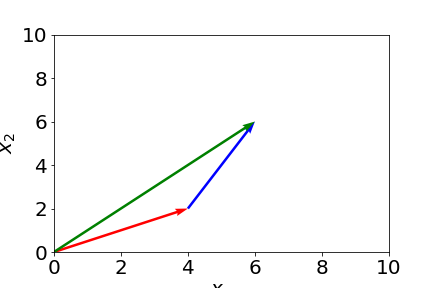
\includegraphics[width=0.9\tw]{images/fig-dist2.png}
  \end{columns}

  \pause
  We want to find the length of vector \colorb{$\w$} where $\alert{\v} + \colorb{\w} = \colorg{\u}$.  Thus,
  \[ \colorb{\w} = \colorg{\u} - \alert{\v} = \colorb{\begin{bmatrix} 2 \\ 4 \end{bmatrix}}. \]

  \bbox
  \[ \colorb{\mbox{dist}(\u,\v) = \| \u - \v \|} = \sqrt{2^2+4^2} = \sqrt{20} \]
  \ebox
\end{frame}


\begin{frame}{Orthogonality}
  \begin{columns}[T]
  \column{0.7\tw}
  Consider two perpendicular vectors $\u$ and $\v$ in $\R^n$.
  \onslide<2->{
  \bi
  \ii We see that $\| \u - \v \| = \| \u - (-\v)\|$.
  \ii Thus $\| \u - \v \|^2 = \| \u - (-\v)\|^2$.
  \ei
  }

  \column{0.3\tw}
  \scalebox{1.0}{
  \begin{tikzpicture}
    \coordinate[label=below left:{$\mathbf{0}$}] (origin) at (0,0) {};
    \coordinate[label=above left:{$\v$}] (v) at (-1,2) {};
    \coordinate[label=above right:{$\u$}] (u) at (2,1) {};
    \draw[->,ultra thick] (origin)--(u);
    \draw[->,ultra thick] (origin)--(v);
    
    \onslide<2->{
    \coordinate[label=below right:{$-\v$}] (minusv) at (1,-2) {};
    \draw[->,ultra thick] (origin)--(minusv);
    \draw[dashed,thick,color=gray] (v)--(u)--(minusv);
    }
  \end{tikzpicture}
  }
  \end{columns}

  \vspace*{-1.4in}

  \pause
  \begin{columns}[T]
  \column{.8\textwidth}
  \blue{
  \begin{align*}
  \onslide<+->{ \| \u - \v \|^2 &= \| \u + \v\|^2\\}
  \onslide<+->{ (\u - \v) \cdot (\u - \v) &= (\u + \v) \cdot (\u + \v)\\}
  \onslide<+->{ \u \cdot (\u - \v) - \v \cdot (\u - \v) &= \u \cdot (\u + \v) + \v \cdot (\u + \v) \\}
  \onslide<+->{ (\u \cdot \u) - (\u \cdot \v) - (\v \cdot \u) + (\v \cdot \v) &= (\u \cdot \u) + (\u \cdot \v) + (\v \cdot \u) + (\v \cdot \v)\\}
  \onslide<+->{ \| \u \|^2 + \| \v \|^2 -2(\u \cdot \v) &= \| \u \|^2 + \| \v \|^2 +2(\u \cdot \v) \\}
  \onslide<+->{ -4(\u \cdot \v) &= 0\\}
  \onslide<+->{ \u \cdot \v &= 0 }
  \end{align*}}
  \column{.2\textwidth}
  \end{columns}
  \vspace*{-2em}

  \onslide<+->{
  \begin{definition}
  Two vectors $\u$ and $\v$ in $\mathbb{R}^n$ are \alert{orthogonal} if and only if \alert{$\u \cdot \v = 0$}.
  \end{definition}
  }
\end{frame}


\begin{frame}{Orthogonality}
  \begin{definition}
  Two vectors $\u$ and $\v$ in $\mathbb{R}^n$ are \alert{orthogonal} if and only if \alert{$\u \cdot \v = 0$}.
  \end{definition}
  \medskip
  
  \blue{Example.}
  \smallskip
  
  \begin{columns}[T]
  \column{.475\textwidth}
  Are $\u=\begin{bmatrix} 5 \\ 2 \end{bmatrix}$ and
      $\v=\begin{bmatrix} -1 \\ 2 \end{bmatrix}$ orthogonal?
  \bigskip
  
  \pause
  \quad $\u \cdot \v = 5(-1) + 2(2) = -1 \alert{\ne 0}$.
  \medskip
  
  $\u$ and $\v$ are \alert{not} orthogonal.
  
  \column{.475\textwidth}
  \pause
  Are $\u=\begin{bmatrix} 4 \\ -7 \\ 2 \end{bmatrix}$ and
      $\v=\begin{bmatrix} -5 \\ -2 \\ 3 \end{bmatrix}$ orthogonal?
  
  \pause
  \begin{align*}
    \u \cdot \v &= 4(-5) + (-7)(-2)+ 2(3) \\
     & = -20+14+6 \alert{=0}.
  \end{align*}

  $\u$ and $\v$ are \alert{orthogonal}.
  \end{columns}
\end{frame}


\begin{frame}{Orthogonal Complements 1}
  \begin{definition}
    If a vector $\mathbf{z}$ is \alert{orthogonal to every vector in a subspace $W$} of $\R^n$, then $\z$ is said to be \alert{orthogonal to $W$}.
    The set of all vectors $\z$ that are orthogonal to $W$ is called the \alert{orthogonal complement of $W$} and is denoted \alert{$W^{\perp}$}.
  \end{definition}

  \begin{columns}[T]
  \column{0.8\tw}
  {\small Consider the plane $W = \mbox{Span} \left\{ \v , \w \right\}$ in $\mathbb{R}^3$ plotted in the figure to the right. }
  \bi
  \ii The vector $\mathbf{z}$ is orthogonal to $W$.
  \ii The orthogonal complement $W^{\perp} = \left\{ c \z \ : \ \mbox{for any scalar } c \right\}$.
  \ei

  \column{0.2\tw}
  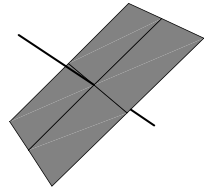
\includegraphics[width=0.9\tw]{images/fig-orthog-comp1.png}
  \end{columns}

%   \pause
%   {\small
%   \bbox
%   \bb
%   \ii A vector $\z$ is in $W^{\perp}$ if and only if $\z$ is orthogonal to \alert{every} vector in a set that \blue{spans} $W$.
%   \ii $W^{\perp}$ is a \alert{subspace} of $\R^n$.
%   \ee
%   \ebox}
\end{frame}


\begin{frame}{Orthogonal Complements 2}
  \begin{theorem}
    Let $W$ be a subspace of $\R^n$.
    Then $W^\perp$ is a \alert{subspace} of $\R^n$.
  \end{theorem}
  \medskip
  
  \pause
  \blue{Proof.}
  We verify the following three properties.
  
  \begin{enumerate}[<+->]
    \item \blue{$W^\perp$ is nonempty.}  Note that $\mathbf{0}$ is orthogonal to every vector in $\R^n$, and so $\mathbf{0}$ is orthogonal to every vector in $W$.  Thus, $\mathbf{0}$ is in $W^\perp$.
    \medskip
    
    \item \blue{$W^\perp$ is closed under addition.}
    Let $\u$ and $\v$ be vectors in $W^\perp$.  Let $\w$ be any vector in $W$.
    \smallskip
    
    Then $\w \cdot (\u+\v) = (\w \cdot \u) + (\w \cdot \v) = 0+0 = 0$.
    Thus, $\u+\v$ is in $W^\perp$.
    \medskip
    
    \item \blue{$W^\perp$ is closed under scalar multiplication.}
    Let $\u$ be a vector in $W^\perp$, and let $c$ be a scalar.
    \smallskip
    
    Let $\w$ be any vector in $W$.
    Then $\w \cdot (c\u) = c(\w \cdot \u)= c0 = 0$.
    Thus, $c\u$ is in $W^\perp$.
    \medskip
  \end{enumerate}
  
  \onslide<5->{
  Thus, $W^\perp$ is a \alert{subspace} of $\R^n$.
  \hfill\blue{$\square$}
  }
\end{frame}


\begin{frame}{Orthogonal Complements 3}
  \begin{theorem}
    Let $W$ be a subspace of $\R^n$.
    A vector $\z$ is in $W^{\perp}$ if and only if $\z$ is orthogonal to \alert{every} vector in a set $\{\v_1,\ldots,\v_p\}$ that \blue{spans} $W$.
  \end{theorem}
  \medskip
  
  \pause
  \blue{Proof.}
  (\blue{$\Rightarrow$}) If $\z$ is in $W^\perp$, then $\z$ is orthogonal to each vector in $W$, including $\v_1,\ldots,\v_p$.
  \bigskip
  
  \pause
  (\blue{$\Leftarrow$})
  Assume that $\z$ is orthogonal to each $\v_i$.
  \smallskip
  
  Let $\w$ be any vector in $W$.
  Since $\{\v_1,\ldots,\v_p\}$ spans $W$,
  there exist scalars $c_1,\ldots,c_p$ such that $\w=c_1 \v_1 + \ldots + c_p \v_p$.
  We compute 
    \[ \z \cdot \w 
      = \z \cdot (c_1 \v_1 + \ldots + c_p \v_p)
      \pause
      = c_1 (\z \cdot \v_1) + \ldots + c_p (\z \cdot \v_p) = 0. \]
  Thus, $\z$ is orthogonal to every vector in $W$, and hence $\z$ is in $W^\perp$.
  \hfill\blue{$\square$}
\end{frame}


\begin{frame}{Matrix Subspaces}
  \medskip

  Let $A = \begin{bmatrix} 1 & 0 & -1 \\ -2 & 0 & 2 \end{bmatrix}$. 
  Find bases for $\Nul A$, $\Col A$, $\Row A$, and $\Nul A^T$.
  \bigskip

  \pause
  \begin{columns}[T]

  \column{0.5\tw}

  We have $\begin{bmatrix} 1 & 0 & -1  \\ -2 & 0 & 2  \end{bmatrix} \xrightarrow{\text{RREF}} \begin{bmatrix} 1 & 0 & -1  \\ 0 & 0 & 0  \end{bmatrix}$.
  \medskip
  
  Thus we have bases
  \begin{align*}
  \Nul A &= \left\{ \begin{bmatrix} 0 \\ 1 \\ 0 \end{bmatrix}, 
                    \begin{bmatrix} 1 \\ 0 \\ 1 \end{bmatrix} \right\} \\[1em]
  \Row A &= \left\{ \begin{bmatrix} 1 & 0 & -1 \end{bmatrix}  \right\} \\[1em]
  \Col A &= \left\{ \begin{bmatrix} 1 \\ -2  \end{bmatrix}  \right\}
  \end{align*}

  \column{0.50\tw}
  \pause
  We have $A^T=\begin{bmatrix} 1 & -2 \\ 0 & 0 \\ -1 & 2 \end{bmatrix} \xrightarrow{\text{RREF}} \begin{bmatrix} 1 & -2 \\ 0 & 0 \\ 0 & 0 \end{bmatrix}$.
  \medskip
  
  Thus we have basis
  \[\Nul A^T = \left\{ \begin{bmatrix} 2 \\ 1  \end{bmatrix} \right\} \]
  \end{columns}
\end{frame}


\begin{frame}{Orthogonal Complement of Matrix Subspaces}
\begin{columns}[T]

\column{0.5\tw}

\begin{example} 
Let $A = \begin{bmatrix} 1 & 0 & -1 \\ -2 & 0 & 2 \end{bmatrix}$. 
\bb
\ii Find a basis for $\Nul A$, $\Col A$ and $\Row A$
\ii Find a basis for $\Nul A^T$.
\ee
\end{example}

We have  bases 

\[ \alert{\Nul A = \left\{ \begin{bmatrix} 0 \\ 1 \\ 0 \end{bmatrix} , \begin{bmatrix} 1 \\ 0 \\ 1 \end{bmatrix} \right\} \quad
 \Row A = \left\{ \begin{bmatrix} 1 \\ 0 \\ -1 \end{bmatrix}  \right\} } \]

\column{0.5\tw}

\[ \colorb{\Col A = \left\{ \begin{bmatrix} 1 \\ -2  \end{bmatrix}  \right\}  \quad \Nul A^T = \left\{ \begin{bmatrix} 2 \\ 1  \end{bmatrix} \right\}}. \]

\begin{center}
%TODO: Right image not correct, plotting span of (2,-1), not (2,1).
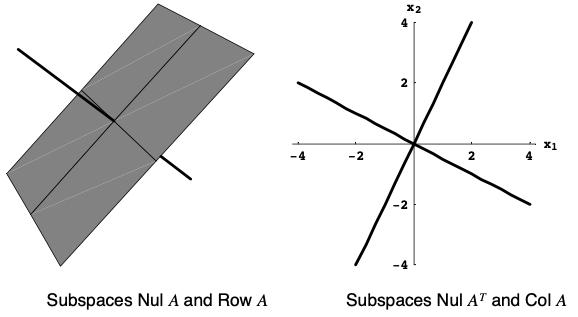
\includegraphics[width=0.95\tw]{images/fig-matrix-subspaces.png}
\end{center}

\end{columns}

\end{frame}


\begin{frame}{Null, Col, and Row Spaces Revisited}
  \begin{theorem}
  Let $A$ be an $m \times n$ matrix. The orthogonal complement of the row space of $A$ is the null space of $A$. The orthogonal complement of the column space of $A$ is the null space of $A^T$.
  \vspace*{-.8em}
  
  \[ (\Row A)^{\perp} = \Nul A \quad \mbox{and} \quad (\Col A)^{\perp} = \Nul A^T\]
  \end{theorem}
  \medskip

  \onslide<2->{
  \blue{Proof.}
  }
  \onslide*<2-6>{
  \vspace*{-.75em}
  
  Let $\x$ be in $(\Row A)^\perp$.
  $A \x = 
      \begin{bmatrix} \mathbf{r}_1 \\  \mathbf{r}_2 \\ \vdots \\  \mathbf{r}_m \end{bmatrix} 
      \begin{bmatrix} x_1 \\ x_2 \\ \vdots \\ x_n \end{bmatrix} =
      \begin{bmatrix} a_{11} & a_{12} & \ldots & a_{1n} \\
                      a_{21} & a_{22} & \ldots & a_{2n} \\
                      \vdots & \vdots & \ddots & \vdots \\
                      a_{m1} & a_{m2} & \ldots & a_{mn} \end{bmatrix}
      \begin{bmatrix} x_1 \\ x_2 \\ \vdots \\ x_n \end{bmatrix}
      \onslide*<3-6>{ = \begin{bmatrix} \mathbf{r}_1 \cdot \x \\  \mathbf{r}_2 \cdot \x \\ \vdots  \\ \mathbf{r}_m \cdot \x \end{bmatrix} }
      \onslide*<4-6>{ = \begin{bmatrix} 0 \\ 0 \\ \vdots \\ 0 \end{bmatrix}.}$%
  \medskip
  }
  
  \onslide*<5-6>{
  Thus $\x$ is in $\Nul A$.
  \smallskip
  
  Similarly, if $\x$ is in $\Nul A$, then it satisfies the equation $A\x = \mathbf{0}$, which implies $\x$ is orthogonal to each row of $A$.
  Since the rows of $A$ span $\Row A$ and by a previous theorem, $\x$ is orthogonal to each vector in $\Row A$.
  Thus, $\x$ is in $(\Row A)^{\perp}$.%
  }%
  \onslide*<6>{
  Therefore we have \blue{$(\Row A)^{\perp} = \Nul A$}.}
  
  \onslide*<7->{
  \medskip
  
  The second statement follows by noting that $\Col A= \Row A^T$:
  \[ (\Col A)^{\perp} = (\Row A^T)^{\perp} = \Nul A^T \]
  
  \vfill\hfill\blue{$\square$}
  }
  
\end{frame}

\end{document}
